%Results body
%Created SS 04-14

\section{Results}\label{results}

\subsection{Observing Optical Pumping and RF Interference}

With the external magnetic field applied, laser light is used to optically pump Rb atoms into a preferential spin state.  To observe this pumping, we measure the fluorescence of pumped Rb atoms using an oscilloscope.  This sample data is shown in Figure \ref{fig:raw_pumping}.

RF interference is used to disrupt the optically pumped steady state by coupling the pumped $m_F$ state to the next (lower) $m_F$ state.  This coupling creates a transient phenomenon which is signified by the decrease in signal from the pumped level to some new steady state.  In order to closely analyze the transient portion due RF interference, a chopped RF signal is used.  
\begin{figure}[htbp]
\begin{center}
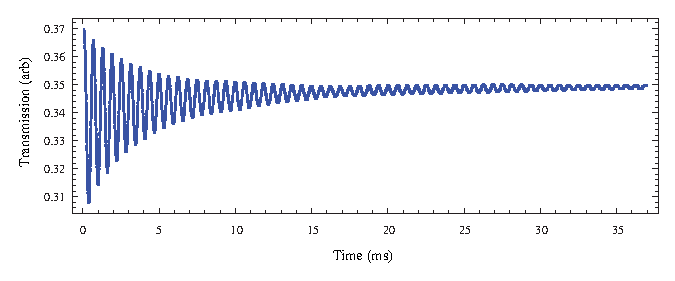
\includegraphics[height=70mm]{./figures/rabi.eps}
\caption{\small{}}
\label{fig:rabi}
\end{center}
\end{figure}
The depumping caused by the $m_F$ coupling combined with optical pumping gives rise to Rabi oscillations in the transient portion between the fully state and the new equilibrium.  This phenomenon is shown in Figure \ref{fig:rabi}.  The oscillations signify periodic fluctuations in spin state populations due to the $m_F$ coupling.    

\subsection{Measuring Linewidth and Optical Pumping Resonance}

Using a lock-in amplifier, we measure the amplitude of Rabi oscillations as a function of applied RF frequency.  We use a \emph{LabVIEW} program in order to select and step through a range of RF frequencies in order to produce a Lorentzian resonance.  This data was taken for both $^{85}$Rb ($F=2$ to $F=2$, $F=3$ to $F=3$ transitions) and $^{87}$Rb ($F=1$ to $F=1$, $F=2$ to $F=2$ transitions).   This data is shown in Figure \ref{fig:rawcurve}.    
\begin{figure}[h!]
\begin{center}
\subfigure[$^{85}$Rb ($F=3$ to $F=3$)]{\label{fig:edge-a}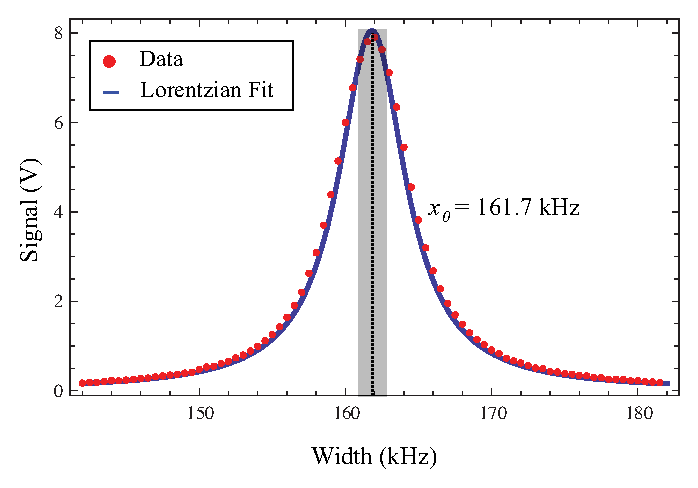
\includegraphics[height=40mm]{./figures/85raw_width.eps}}
\hspace{-1mm}
\vspace{-2mm}
\subfigure[$^{87}$Rb ($F=2$ to $F=2$)]{\label{fig:edge-b}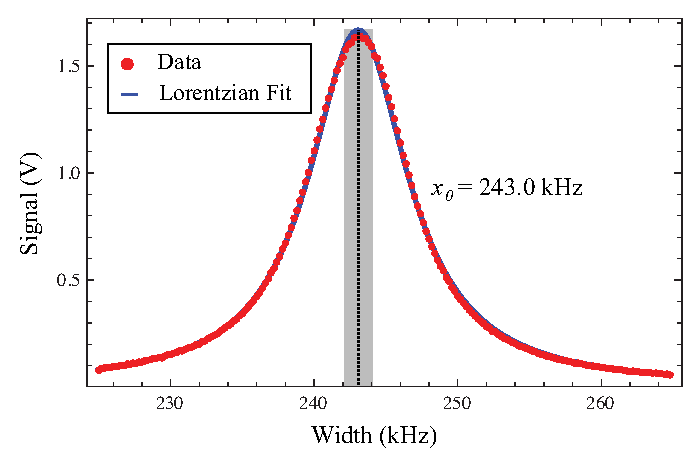
\includegraphics[height=40mm]{./figures/87raw_width.eps}}
\vspace{-2mm}
\caption{\small{}}
\label{fig:rawcurve}
\end{center}
\end{figure}
This data was fit to lorentzian distributions.  These fits were then used to calculate the center, or resonant,  frequencies.  The resonant $m_F$ coupling frequencies for $^{85}$Rb and $^{87}$Rb are $161.7$ kHz and $243.0$ kHz respectively.  

Further measurements are taken using the $^{85}$Rb $F=3$ to $F=3$ transition to determine the effect of RF amplitude and laser light intensity on the linewidth of the resonance. By independently varying either of these variables, several resonances are measured.  Using a \emph{Mathematica} program, the linewidths of these resonances are calculated and plotted with respect to both RF amplitude and laser light intensity.  This data is shown in Figure \ref{fig:linewidths}.
\begin{figure}[h!]
\begin{center}
\subfigure[Varying RF Amplitude]{\label{fig:edge-a}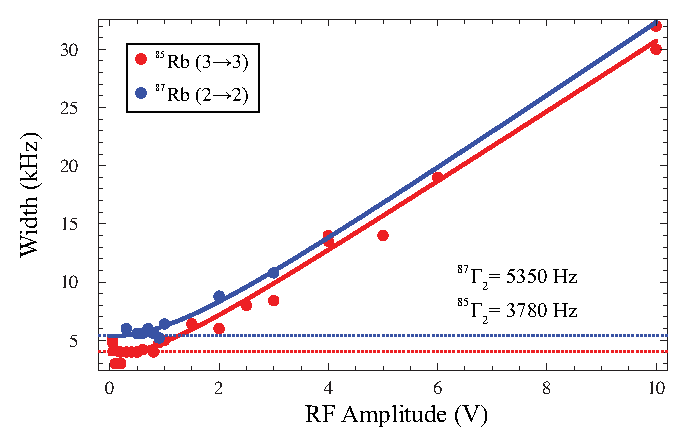
\includegraphics[height=40mm]{./figures/amp_width.eps}}
\hspace{-1mm}
\vspace{-2mm}
\subfigure[Varying Intensity]{\label{fig:edge-b}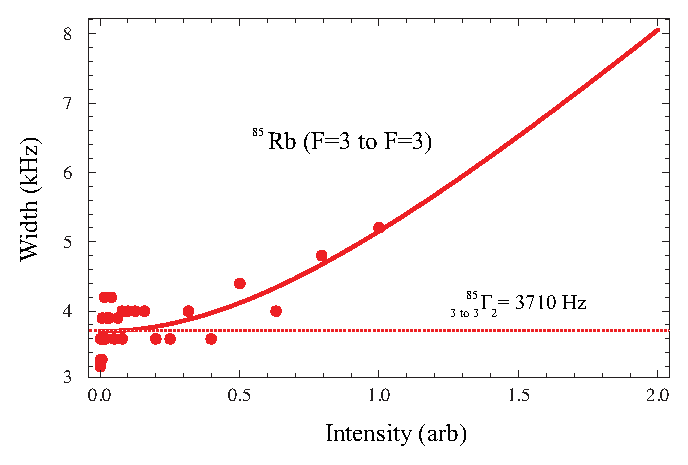
\includegraphics[height=40mm]{./figures/intensity_width.eps}}
\vspace{-2mm}
\caption{\small{}}
\label{fig:linewidths}
\end{center}
\end{figure}
The variable being held constant was held constant in a regime in which it would not have a confounding effect on the linewidth (\emph{i.e.} while varying light intensity, RF amplitude was minimized and \emph{vice versa}).  We expect the linewidth to be given by 
\begin{center}
\begin{equation}\label{linewidth}
\gamma=\gamma_0\sqrt{1+\kappa}
\end{equation}
\end{center}
where $\gamma_0$ is the natural linewidth and $\kappa \propto \mathcal E_0^{2}$ where $\mathcal E_0$ is the amplitude of the light electric field.  Accordingly, the data for varying RF amplitude (proportional to $\cal E_0$) is fit to a $\alpha \sqrt{1+\beta x^2}$ model whereas the data for varying light intensity (proportional to $\mathcal E_0^{2}$) is fit to a $\alpha \sqrt{1+\beta x^2}$ model.  Both fits are done using nonlinear regression analysis (See Appendix \ref{nonlinearregression}).  We would expect the natural linewidths for each measurement process to be the same.  From our fitting analysis we find the natural linewidths to be $3.78 \pm BLAH$ Hz and $3.63 \pm BLAH$ Hz for varying RF amplitude and light intensity respectively.  Given the error for this measurement, the two values are in good agreement. 

\subsection{Measuring}

\begin{figure}[htbp]
\begin{center}
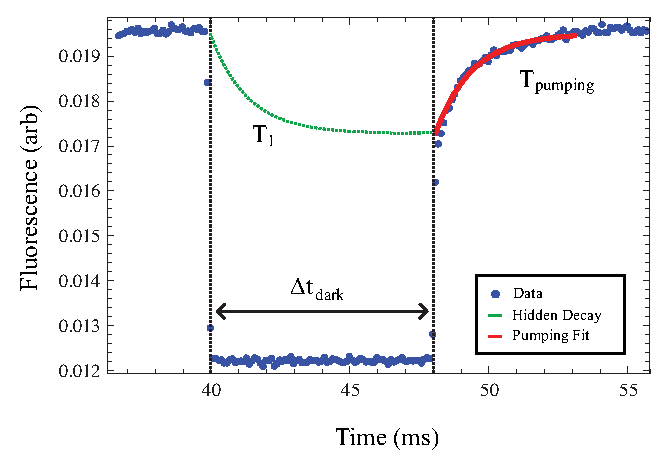
\includegraphics[height=70mm]{./figures/raw_chop.eps}
\caption{\small{}}
\label{fig:chop}
\end{center}
\end{figure}

\subsection{Measuring Spin Exchange Between $^{85}$Rb and $^{87}$Rb}